\documentclass[aspectratio=169,11pt]{beamer}

\usepackage[T1]{fontenc}
\usepackage{lmodern}
\usepackage{graphicx}
\usepackage{booktabs}
\usepackage{tabularx}
\usepackage{array}
\usepackage{tikz}
\usepackage{xurl}
\usetikzlibrary{arrows.meta,positioning,fit}

\definecolor{kublue}{RGB}{23,37,84}
\definecolor{kugold}{RGB}{250,204,21}
\definecolor{softblue}{RGB}{239,246,255}
\definecolor{softgreen}{RGB}{236,253,245}
\definecolor{softred}{RGB}{254,242,242}
\definecolor{textgray}{RGB}{51,65,85}

\usetheme{default}
\usecolortheme{default}
\setbeamercolor{palette primary}{bg=kublue,fg=white}
\setbeamercolor{palette secondary}{bg=kublue,fg=white}
\setbeamercolor{palette tertiary}{bg=kublue,fg=white}
\setbeamercolor{frametitle}{bg=kublue,fg=white}
\setbeamercolor{title}{fg=white,bg=kublue}
\setbeamercolor{block title}{bg=kublue,fg=white}
\setbeamercolor{block body}{bg=softblue,fg=black}
\setbeamercolor{alerted text}{fg=red!75!black}
\setbeamertemplate{headline}{}
\setbeamertemplate{navigation symbols}{}
\setbeamertemplate{footline}{}
\setbeamertemplate{itemize item}{\color{kugold}$\blacktriangleright$}
\setbeamertemplate{itemize subitem}{\color{kublue}$\bullet$}

\newcolumntype{Y}{>{\raggedright\arraybackslash}X}
\newcommand{\projecttitle}{MarketGyan: NEPSE and Financial News Analysis}
\newcommand{\studentsname}{Bikash Kumar Sah}
\newcommand{\rollnumber}{16}
\newcommand{\supervisorone}{Mr. Sundeep Gupta}
\newcommand{\supervisortwo}{Ms. Sristi Khatiwada}
\newcommand{\departmentname}{Department of Artificial Intelligence}
\newcommand{\universityname}{Kathmandu University}
\newcommand{\submissiondate}{July 6, 2026}
\pdfstringdefDisableCommands{\def\\{ }}

\title[\projecttitle]{\projecttitle}
\subtitle{An Extension of Khabar AI}
\author{\studentsname \\ Roll No.: \rollnumber}
\institute{\departmentname \\ \universityname}
\date{\submissiondate}
\hypersetup{
  pdftitle={MarketGyan: NEPSE and Financial News Analysis},
  pdfauthor={Bikash Kumar Sah}
}

\begin{document}

\begin{frame}[plain]
  \vspace{0.18cm}
  \begin{center}
    {\Large\bfseries \universityname}\\[0.06cm]
    {\normalsize School of Engineering}\\
    {\normalsize \departmentname}\\[0.34cm]
    {\small\bfseries Final Year Project Presentation}\\[0.18cm]
    \colorbox{kublue}{%
      \parbox{0.84\paperwidth}{\centering
        \vspace{0.22cm}
        {\color{white}\Large\bfseries MarketGyan}\\[0.08cm]
        {\color{white}\normalsize NEPSE and Financial News Analysis}\\
        {\color{white}\small An Extension of Khabar AI}
        \vspace{0.22cm}
      }}
    \\[0.45cm]
    \begin{tabular}{@{}rl@{}}
      \textbf{Presented by:} & \studentsname \\
      \textbf{Roll No.:} & \rollnumber \\
      \textbf{Supervised by:} & \supervisorone \\
                              & \supervisortwo \\
      \textbf{Department:} & \departmentname \\
      \textbf{Date:} & \submissiondate \\
    \end{tabular}
  \end{center}
\end{frame}

\begin{frame}{Outline}
  \begin{columns}[T,onlytextwidth]
    \begin{column}{0.48\textwidth}
      \begin{enumerate}
        \item Introduction and motivation
        \item Objectives and scope
        \item Literature review
        \item Proposed system and architecture
        \item Methodology and Schema-v2
      \end{enumerate}
    \end{column}
    \begin{column}{0.48\textwidth}
      \begin{enumerate}
        \setcounter{enumi}{5}
        \item Tools and implementation
        \item Results and evaluation
        \item Limitations and future work
        \item Conclusion and references
      \end{enumerate}
    \end{column}
  \end{columns}
\end{frame}

\begin{frame}{Introduction}
  \begin{block}{Project idea}
    MarketGyan extends Khabar AI into a Nepal-focused financial NLP assistant for NEPSE-related news, evidence search, and grounded market reports.
  \end{block}

  \begin{itemize}
    \item Connects market snapshots, financial news, and policy documents.
    \item Classifies whether a story is directly relevant, indirectly relevant, or not relevant to NEPSE.
    \item Produces structured impact fields: event type, direction, sector, symbol, mechanism, and evidence sentence IDs.
    \item Uses RAG so current facts remain in retrieved evidence rather than model weights.
  \end{itemize}
\end{frame}

\begin{frame}{Motivation and Background}
  \begin{columns}[T,onlytextwidth]
    \begin{column}{0.53\textwidth}
      \textbf{Why this matters}
      \begin{itemize}
        \item NEPSE data, financial news, and regulatory updates are scattered across many sources.
        \item Investors must manually connect market movement with related events.
        \item Generic news summarizers do not know NEPSE-specific symbols, sectors, and event taxonomy.
      \end{itemize}
    \end{column}
    \begin{column}{0.43\textwidth}
      \begin{block}{Need for the system}
        A Nepal-specific assistant should answer with source-backed evidence, not generic positive or negative tone.
      \end{block}
      \begin{alertblock}{Safety boundary}
        Informational analysis only. No buy/sell advice.
      \end{alertblock}
    \end{column}
  \end{columns}
\end{frame}

\begin{frame}{Project Objectives}
  \begin{block}{Main objective}
    Build and evaluate a Nepal-specific financial news analysis system that combines structured NEPSE data, financial-news retrieval, and a fine-tuned instruction model.
  \end{block}

  \textbf{Specific objectives}
  \begin{enumerate}
    \item Collect and manage NEPSE-related market data, financial news, and selected regulatory sources.
    \item Create a bilingual, evidence-grounded NEPSE impact benchmark.
    \item Fine-tune and evaluate Qwen3.5-9B LoRA for compact structured impact extraction.
    \item Build a RAG runtime for grounded query answering and report generation.
  \end{enumerate}
\end{frame}

\begin{frame}{Scope of the Project}
  \begin{columns}[T,onlytextwidth]
    \begin{column}{0.48\textwidth}
      \begin{block}{Included}
        \begin{itemize}
          \item Public NEPSE snapshots and finance news.
          \item English and Nepali article processing.
          \item NEPSE-Impact-500 dataset.
          \item Qwen3.5-9B LoRA adapter.
          \item Evidence search, Ask MarketGyan, and report generation.
        \end{itemize}
      \end{block}
    \end{column}
    \begin{column}{0.48\textwidth}
      \begin{alertblock}{Not included}
        \begin{itemize}
          \item Brokerage integration or order execution.
          \item Personalized investment advice.
          \item Trading prediction or causal market forecasting.
          \item Production deployment until retrieval and content gates pass.
        \end{itemize}
      \end{alertblock}
    \end{column}
  \end{columns}
\end{frame}

\begin{frame}{Literature Review: Financial NLP}
  \begin{block}{FinBERT}
    FinBERT shows that adapting transformer models to financial text improves financial sentiment classification compared with generic language models.
  \end{block}
  \begin{itemize}
    \item Useful lesson: financial words are event- and domain-dependent.
    \item MarketGyan gap: NEPSE analysis needs more than positive/negative sentiment.
    \item Required fields include relevance, event type, impact scope, direction, sector, symbol, and evidence.
  \end{itemize}
\end{frame}

\begin{frame}{Literature Review: Financial LLMs}
  \begin{tabularx}{\textwidth}{@{}lY@{}}
    \toprule
    Study & Relevance to MarketGyan \\
    \midrule
    FinGPT & Supports a data-centric approach: curate financial data and adapt a moderate-size model with lightweight tuning. \\
    FinLLM survey & Highlights hallucination risk, benchmark weakness, and the need to separate validity, grounding, and task metrics. \\
    FinTral & Demonstrates financial instruction tuning for multi-task structured outputs on a moderately sized open model. \\
    \bottomrule
  \end{tabularx}

  \vspace{0.24cm}
  \begin{block}{Adopted design}
    MarketGyan treats the Nepal-specific ontology and evidence-grounded benchmark as the main contribution; LoRA is the adaptation method, not the novelty.
  \end{block}
\end{frame}

\begin{frame}{Literature Review: Nepali NLP}
  \begin{tabularx}{\textwidth}{@{}lY@{}}
    \toprule
    Work & Relevance and limitation \\
    \midrule
    NepBERTa & Shows that Nepali-specific pre-training improves Nepali NLP tasks. \\
    Subedi et al. & Evaluates LLMs for Nepali NER and POS tagging, showing promise but also low-resource benchmark gaps. \\
    Thapa et al. & Expands Nepali transformer resources with larger monolingual pre-training for understanding and generation. \\
    \bottomrule
  \end{tabularx}

  \vspace{0.24cm}
  \begin{alertblock}{Gap}
    These works are not finance-specific. MarketGyan therefore builds a bilingual NEPSE benchmark instead of relying only on general Nepali NLP resources.
  \end{alertblock}
\end{frame}

\begin{frame}{Proposed System Overview}
  \begin{columns}[T,onlytextwidth]
    \begin{column}{0.52\textwidth}
      \textbf{Core pipeline}
      \begin{enumerate}
        \item Collect market/news/policy data.
        \item Normalize and index finance evidence.
        \item Retrieve candidate evidence for a query or report date.
        \item Ask Qwen3.5-9B for compact structured output.
        \item Materialize citations from retrieved rows.
      \end{enumerate}
    \end{column}
    \begin{column}{0.44\textwidth}
      \begin{block}{Final runtime decision}
        Single-pass RAG replaced the earlier context-heavy multi-agent prompt because it passed live citation checks without exceeding the vLLM context limit.
      \end{block}
    \end{column}
  \end{columns}
\end{frame}

\begin{frame}{Training and Evaluation Workflow}
  \centering
  \resizebox{0.97\textwidth}{!}{%
  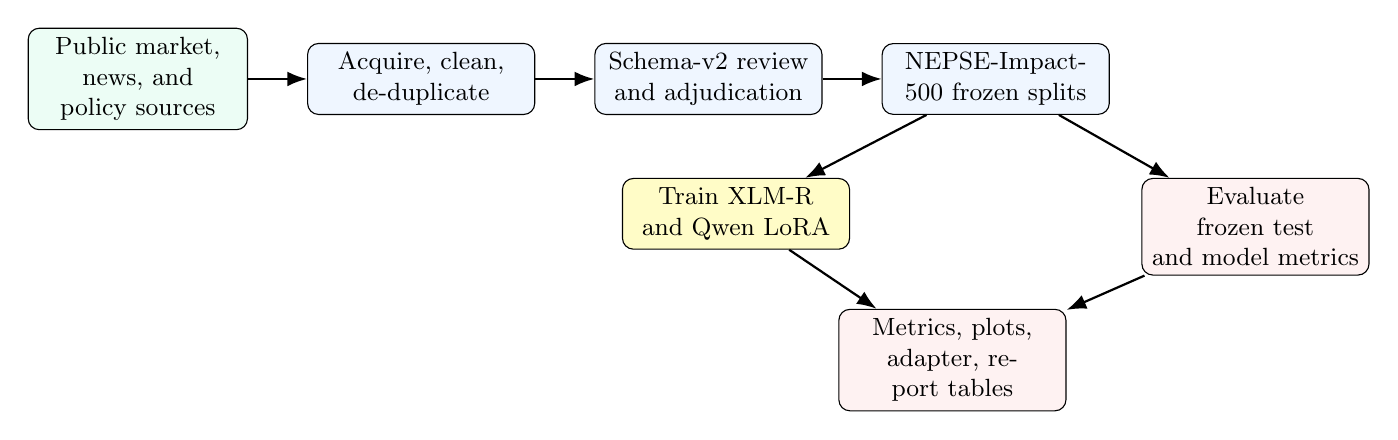
\begin{tikzpicture}[
      node distance=0.75cm,
      every node/.style={font=\small},
      source/.style={draw, rounded corners, align=center, text width=2.55cm, minimum height=0.86cm, fill=softgreen},
      process/.style={draw, rounded corners, align=center, text width=2.65cm, minimum height=0.86cm, fill=softblue},
      model/.style={draw, rounded corners, align=center, text width=2.65cm, minimum height=0.86cm, fill=yellow!22},
      output/.style={draw, rounded corners, align=center, text width=2.65cm, minimum height=0.86cm, fill=softred},
      arrow/.style={-{Latex[length=2.5mm]}, thick}
  ]
    \node[source] (sources) {Public market, news, and policy sources};
    \node[process, right=of sources] (acq) {Acquire, clean, de-duplicate};
    \node[process, right=of acq] (review) {Schema-v2 review and adjudication};
    \node[process, right=of review] (splits) {NEPSE-Impact-500 frozen splits};
    \node[model, below left=0.8cm and 0.4cm of splits] (train) {Train XLM-R and Qwen LoRA};
    \node[output, below right=0.8cm and 0.4cm of splits] (eval) {Evaluate frozen test and model metrics};
    \node[output, below right=0.75cm and -0.15cm of train] (artifacts) {Metrics, plots, adapter, report tables};
    \draw[arrow] (sources) -- (acq);
    \draw[arrow] (acq) -- (review);
    \draw[arrow] (review) -- (splits);
    \draw[arrow] (splits) -- (train);
    \draw[arrow] (splits) -- (eval);
    \draw[arrow] (train) -- (artifacts);
    \draw[arrow] (eval) -- (artifacts);
  \end{tikzpicture}}

  \vspace{0.25cm}
  \small The frozen benchmark keeps model comparison separate from live retrieval and frontend behavior.
\end{frame}

\begin{frame}{Daily Inference Workflow}
  \centering
  \resizebox{0.98\textwidth}{!}{%
  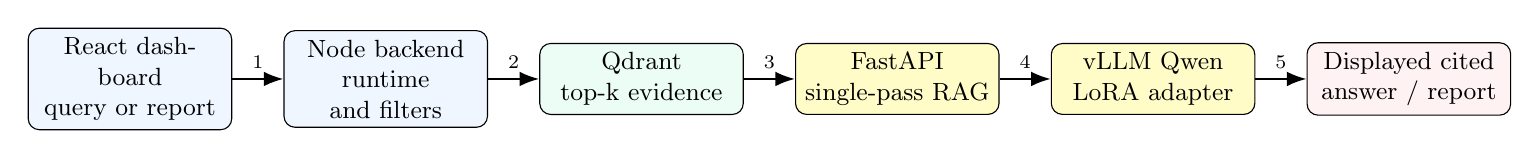
\begin{tikzpicture}[
      node distance=0.65cm,
      every node/.style={font=\small},
      flowstep/.style={draw, rounded corners, align=center, text width=2.35cm, minimum height=0.9cm, fill=softblue},
      store/.style={draw, rounded corners, align=center, text width=2.35cm, minimum height=0.9cm, fill=softgreen},
      model/.style={draw, rounded corners, align=center, text width=2.35cm, minimum height=0.9cm, fill=yellow!22},
      output/.style={draw, rounded corners, align=center, text width=2.35cm, minimum height=0.9cm, fill=softred},
      arrow/.style={-{Latex[length=2.5mm]}, thick}
  ]
    \node[flowstep] (ui) {React dashboard\\query or report};
    \node[flowstep, right=of ui] (node) {Node backend\\runtime and filters};
    \node[store, right=of node] (qdrant) {Qdrant\\top-k evidence};
    \node[model, right=of qdrant] (agent) {FastAPI\\single-pass RAG};
    \node[model, right=of agent] (vllm) {vLLM Qwen\\LoRA adapter};
    \node[output, right=of vllm] (answer) {Displayed cited\\answer / report};
    \draw[arrow] (ui) -- node[above, font=\scriptsize] {1} (node);
    \draw[arrow] (node) -- node[above, font=\scriptsize] {2} (qdrant);
    \draw[arrow] (qdrant) -- node[above, font=\scriptsize] {3} (agent);
    \draw[arrow] (agent) -- node[above, font=\scriptsize] {4} (vllm);
    \draw[arrow] (vllm) -- node[above, font=\scriptsize] {5} (answer);
  \end{tikzpicture}}

  \vspace{0.25cm}
  \small Citations are reconstructed from retrieved evidence rows with URL, excerpt, content hash, chunk ID, and sentence IDs.
\end{frame}

\begin{frame}{Methodology I: Data and Schema-v2}
  \begin{columns}[T,onlytextwidth]
    \begin{column}{0.50\textwidth}
      \begin{block}{Data pipeline}
        \begin{itemize}
          \item Acquire public NEPSE snapshots, financial news, and selected machine-readable policy text.
          \item Clean, de-duplicate, sentence-split, and attach stable URLs/content hashes.
          \item Review generated candidates and export only adjudicated gold labels.
        \end{itemize}
      \end{block}
    \end{column}
    \begin{column}{0.47\textwidth}
      \begin{block}{Benchmark}
        \begin{itemize}
          \item NEPSE-Impact-500: 300 direct, 100 indirect, 100 hard negatives.
          \item Frozen split: 350 train, 75 validation, 75 test.
          \item Duplicate groups stay inside the same split to prevent leakage.
        \end{itemize}
      \end{block}
    \end{column}
  \end{columns}
\end{frame}

\begin{frame}[fragile]{Methodology II: Schema-v2 JSON Contract}
  \scriptsize
  \begin{verbatim}
{
  "relevance": "direct | indirect | not_relevant",
  "eventType": "market_trading | earnings | regulation | governance |
                credit_financing | capital_action | sector_industry |
                project_operations | macro_policy | other | none",
  "impactScope": "market | sector | company | not_applicable",
  "impactDirection": "bullish | bearish | neutral | uncertain |
                      not_applicable",
  "sectors": ["Banking"],
  "symbols": ["NABIL"],
  "rationale": "short evidence-based reason",
  "confidenceBand": "low | medium | high",
  "evidenceSentenceIds": ["S1", "S3"]
}
  \end{verbatim}
  \vspace{-0.05cm}
  \begin{block}{Validation rule}
    Evidence IDs must point to real numbered source sentences. Relevant rows need defensible impact fields; not-relevant rows must not invent sectors, symbols, or market impact.
  \end{block}
\end{frame}

\begin{frame}{Methodology III: Modeling and Runtime Evaluation}
  \begin{columns}[T,onlytextwidth]
    \begin{column}{0.49\textwidth}
      \textbf{Modeling}
      \begin{itemize}
        \item XLM-R relevance and direction baselines.
        \item English-only FinBERT sanity baseline.
        \item Base Qwen zero-shot and three-shot ablations.
        \item Qwen3.5-9B BF16 LoRA targeted-v2 final adapter.
      \end{itemize}
    \end{column}
    \begin{column}{0.49\textwidth}
      \textbf{Evaluation}
      \begin{itemize}
        \item Frozen test split for model metrics.
        \item Strict structured validity and evidence grounding gates.
        \item Per-class F1 for relevance and merged direction.
        \item vLLM JSON Schema constrained inference check.
      \end{itemize}
    \end{column}
  \end{columns}
\end{frame}

\begin{frame}{System Requirements and Training Setup}
  \small
  \begin{tabularx}{\textwidth}{@{}lY@{}}
    \toprule
    Area & Final setup from report \\
    \midrule
    Local runtime & React, Node/Express, MongoDB, Qdrant, Python FastAPI agent. \\
    Model serving & Lightning AI Studio with vLLM OpenAI-compatible endpoint. \\
    XLM-R baseline & \texttt{xlm-roberta-base}, 512 tokens, LR \(2e{-5}\), max 8 epochs, class-weighted loss, validation macro-F1 selection. \\
    Qwen training & \texttt{Qwen/Qwen3.5-9B}, BF16 LoRA, rank 32, alpha 64, max sequence 2048, LR \(2e{-5}\), 3 epochs, A100 80GB. \\
    Safety & Local report generation, citation validation, disclaimer, no buy/sell advice. \\
    \bottomrule
  \end{tabularx}
\end{frame}

\begin{frame}{Qwen3.5-9B Training Configuration}
  \scriptsize
  \begin{tabularx}{\textwidth}{@{}lYlY@{}}
    \toprule
    Item & Value & Item & Value \\
    \midrule
    Base model & \texttt{Qwen/Qwen3.5-9B} & Precision & BF16 LoRA, no 4-bit \\
    Max sequence & 2048 & Max generation & 256 tokens \\
    LoRA & rank 32, alpha 64, dropout 0.05 & Epochs & 3 \\
    Batch & train/eval 4 & Grad accumulation & 2 \\
    Learning rate & \(2e{-5}\) & Optimizer & \texttt{paged\_adamw\_8bit} \\
    Checkpointing & eval/save every 10 steps & Best model & validation loss \\
    Oversampling & \texttt{targeted\_v2} & Train rows & 350 to 922 weighted examples \\
    Output & \multicolumn{3}{l}{\begin{tabular}[t]{@{}l@{}}\texttt{marketgyan-qwen35-9b-a100-80gb}\\\texttt{-bf16-lora-targeted-v2}\end{tabular}} \\
    \bottomrule
  \end{tabularx}

  \vspace{0.22cm}
  \begin{block}{Reason for this setup}
    The latest run optimized content metrics while preserving strict JSON validity and evidence grounding; the frozen test split was not used for oversampling.
  \end{block}
\end{frame}

\begin{frame}{Tools and Technologies}
  \begin{tabularx}{\textwidth}{@{}lY@{}}
    \toprule
    Layer & Tools used \\
    \midrule
    Frontend & React dashboard with MarketGyan tabs: Overview, Ask, Evidence Search, Reports, System. \\
    Backend & Node.js / Express APIs, MongoDB, scheduler, report persistence, review tools. \\
    Retrieval & Qdrant vector database with finance-specific evidence payloads. \\
    ML service & Python, FastAPI, evaluation CLI, schema validators. \\
    Model training & Qwen3.5-9B, LoRA, BF16 training, A100 80GB, frozen test split. \\
    Model serving & Lightning AI Studio, vLLM OpenAI-compatible endpoint, JSON Schema constrained decoding. \\
    \bottomrule
  \end{tabularx}
\end{frame}

\begin{frame}{Implementation Details}
  \begin{columns}[T,onlytextwidth]
    \begin{column}{0.49\textwidth}
      \begin{block}{Backend and data modules}
        \begin{itemize}
          \item Article, market snapshot, market document, security, and report records.
          \item Candidate generation, review, adjudication, and schema validation.
          \item Runtime status, protected report generation, scheduler, and persistence.
          \item React tabs for Overview, Ask, Evidence Search, Reports, System, and validation.
        \end{itemize}
      \end{block}
    \end{column}
    \begin{column}{0.49\textwidth}
      \begin{block}{ML and runtime modules}
        \begin{itemize}
          \item XLM-R baseline training and Qwen LoRA notebook/script pipeline.
          \item Qdrant finance-evidence indexer with source URL, content hash, chunk ID, and sentence IDs.
          \item FastAPI single-pass RAG agent for grounded answers and reports.
          \item Evaluation CLI for frozen model metrics, retrieval labels, and live scenarios.
        \end{itemize}
      \end{block}
    \end{column}
  \end{columns}
\end{frame}

\begin{frame}{Results: 4-bit QLoRA vs 16-bit BF16 LoRA}
  \scriptsize
  \renewcommand{\arraystretch}{0.92}
  \begin{tabularx}{\textwidth}{@{}lccY@{}}
    \toprule
    Metric & 4-bit QLoRA & 16-bit BF16 LoRA & Status \\
     & (Qwen3-8B) & (Qwen3.5-9B v2) & \\
    \midrule
    Structured validity & 0.360 & 1.000 & 16-bit passes 0.95 gate \\
    Evidence grounding & 0.360 & 1.000 & 16-bit passes 0.95 gate \\
    Relevance macro-F1 & 0.384 & 0.796 & Pass \\
    Nepali relevance acc. & 0.182 & 0.788 & Large gain \\
    Event macro-F1 & --- & 0.633 & Below 0.65 \\
    Direction macro-F1 & 0.413 & 0.575 & Below 0.65 \\
    Sector micro-F1 & --- & 0.677 & Below target \\
    Symbol micro-F1 & --- & 0.793 & Near target \\
    Evidence sentence F1 & --- & 0.736 & Below target \\
    \bottomrule
  \end{tabularx}

  \vspace{0.08cm}
  {\tiny 4-bit column is the final (v3) Qwen3-8B QLoRA diagnostic run; earlier runs scored 0.413 and 0.347 strict validity.}

  \vspace{0.04cm}
  \begin{alertblock}{Why 16-bit BF16 LoRA is the final candidate}
    QLoRA stayed near 0.35--0.41 strict validity and grounding, below the 0.95 gate. BF16 LoRA reached 1.000 on both and improved Nepali relevance; event, direction, sector, and evidence metrics still need work.
  \end{alertblock}
\end{frame}

\begin{frame}{Baseline and Qwen Ablation Results}
  \scriptsize
  \begin{columns}[T,onlytextwidth]
    \begin{column}{0.46\textwidth}
      \textbf{Supervised baselines}
      \begin{tabular}{@{}lcc@{}}
        \toprule
        Model / task & Acc. & Macro-F1 \\
        \midrule
        XLM-R relevance & 0.813 & 0.743 \\
        XLM-R direction & 0.567 & 0.568 \\
        FinBERT direction & 0.889 & 0.616 \\
        \bottomrule
      \end{tabular}
      \vspace{0.18cm}

      \scriptsize XLM-R direction uses the merged neutral-or-uncertain target; FinBERT support is small and English-only.
    \end{column}
    \begin{column}{0.50\textwidth}
      \textbf{Qwen conditions}
      \begin{tabular}{@{}lccc@{}}
        \toprule
        Condition & Valid & Rel. F1 & Evid. F1 \\
        \midrule
        Zero-shot & 0.000 & 0.367 & 0.000 \\
        Three-shot & 0.987 & 0.435 & 0.599 \\
        Targeted-v2 LoRA & 1.000 & 0.796 & 0.736 \\
        \bottomrule
      \end{tabular}
      \vspace{0.18cm}

      \scriptsize Fine-tuning solves strict structure/grounding and improves relevance, but neutral direction remains weak.
    \end{column}
  \end{columns}
\end{frame}

\begin{frame}{XLM-R Relevance Baseline}
  \centering
  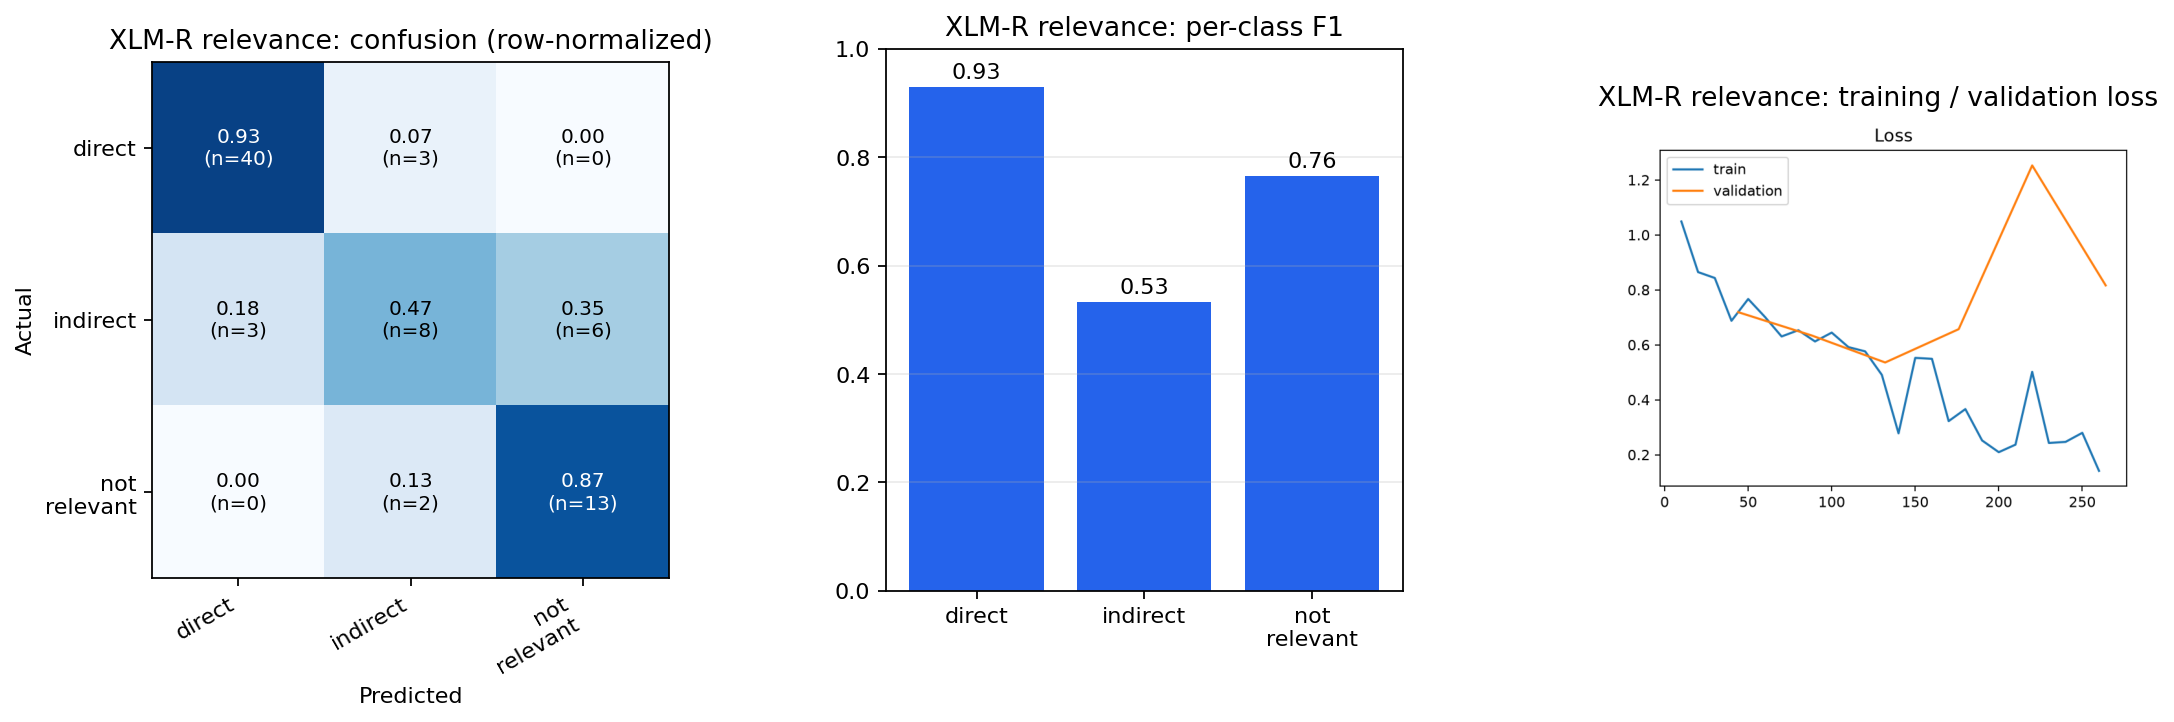
\includegraphics[width=\textwidth]{assets/xlmr-relevance-combined.png}

  \vspace{0.12cm}
  \small XLM-R relevance: accuracy 0.813, macro-F1 0.743 on the frozen test split. Row-normalized confusion, per-class F1, and the training/validation loss curve.
\end{frame}

\begin{frame}{XLM-R Direction Baseline}
  \centering
  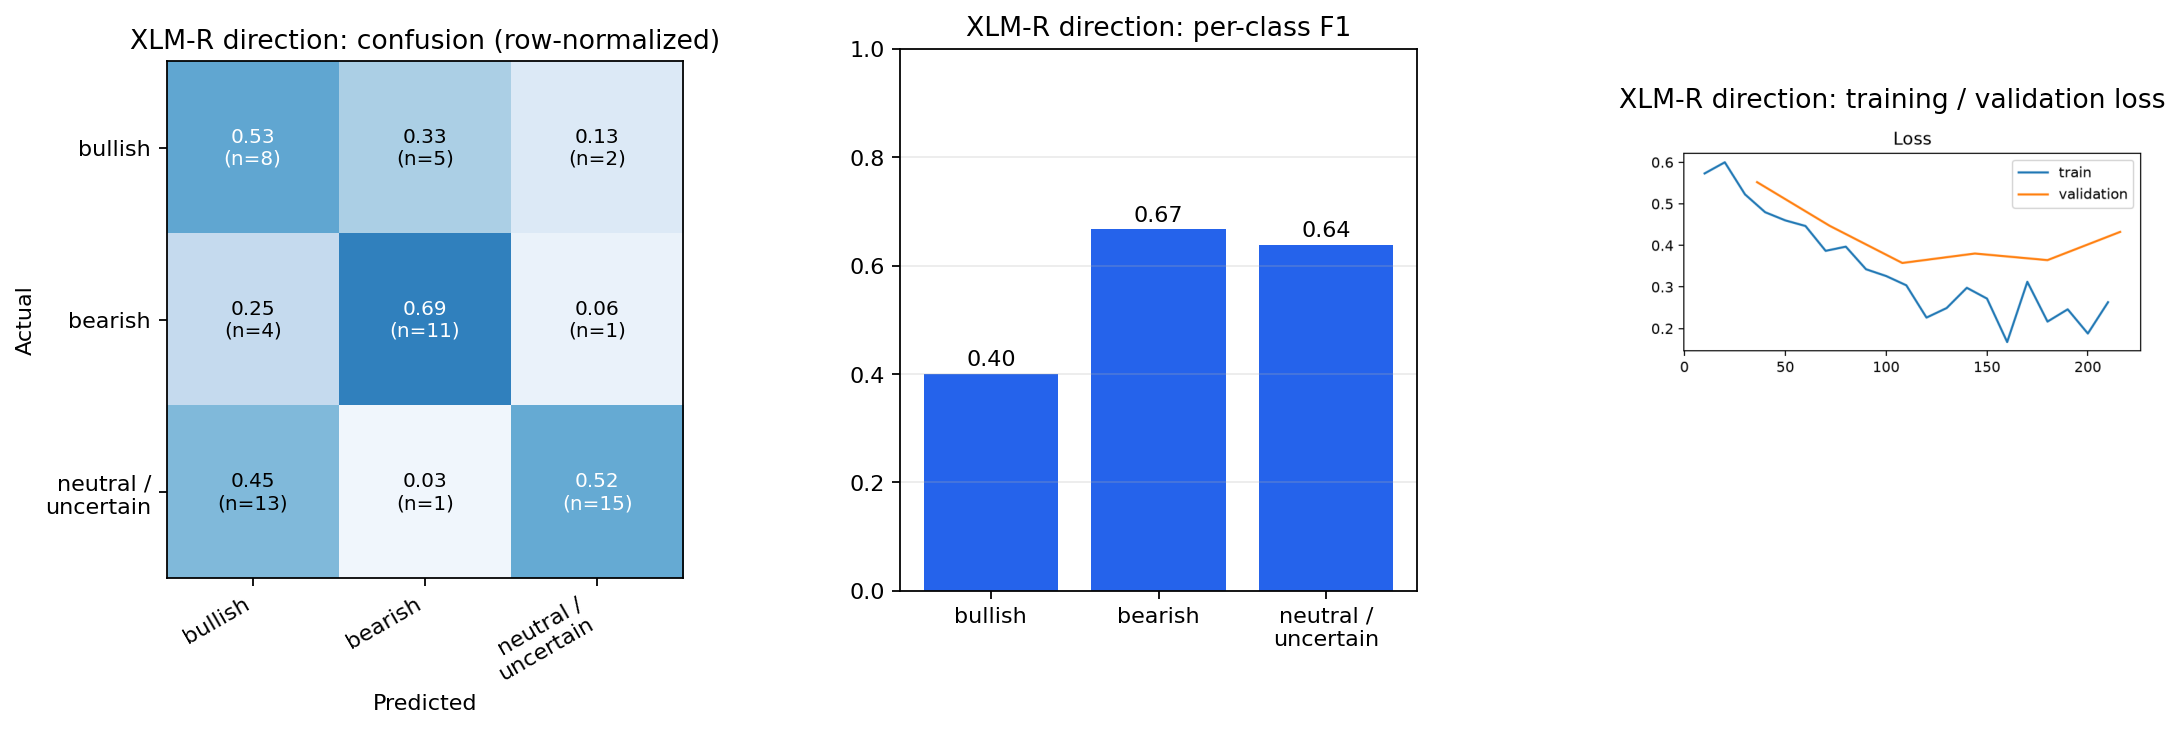
\includegraphics[width=\textwidth]{assets/xlmr-direction-combined.png}

  \vspace{0.12cm}
  \small XLM-R direction (merged neutral-or-uncertain): accuracy 0.567, macro-F1 0.568 on relevant frozen-test rows. Merging avoids the unlearnable standalone neutral class and leaves no dead class.
\end{frame}

\begin{frame}{Qwen Targeted-v2 Loss Curve}
  \centering
  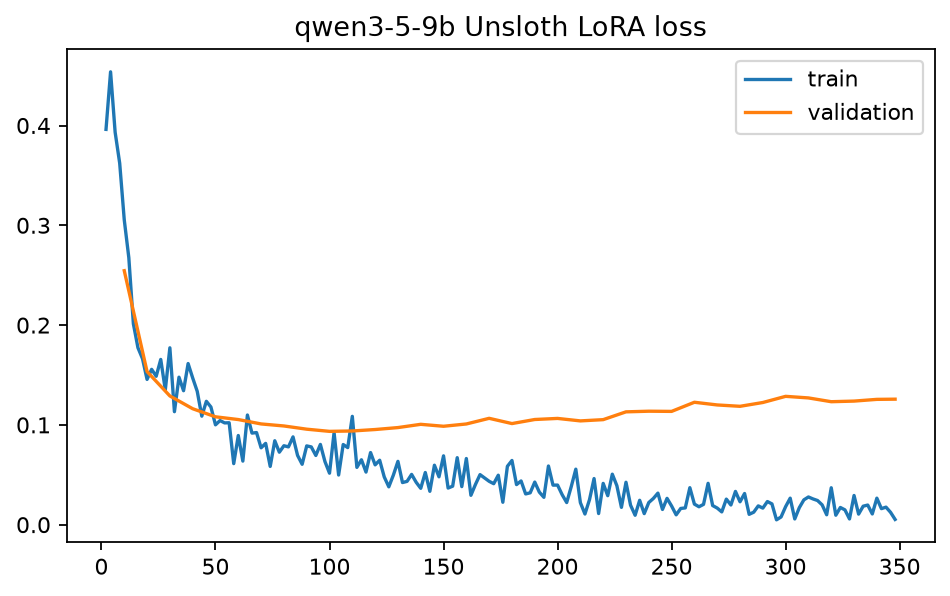
\includegraphics[height=0.72\textheight]{assets/loss.png}

  \vspace{0.12cm}
  \small Validation loss flattens and rises after early improvement, supporting best-checkpoint selection instead of longer blind training.
\end{frame}

\begin{frame}{Qwen Targeted-v2 Test Result Plot}
  \centering
  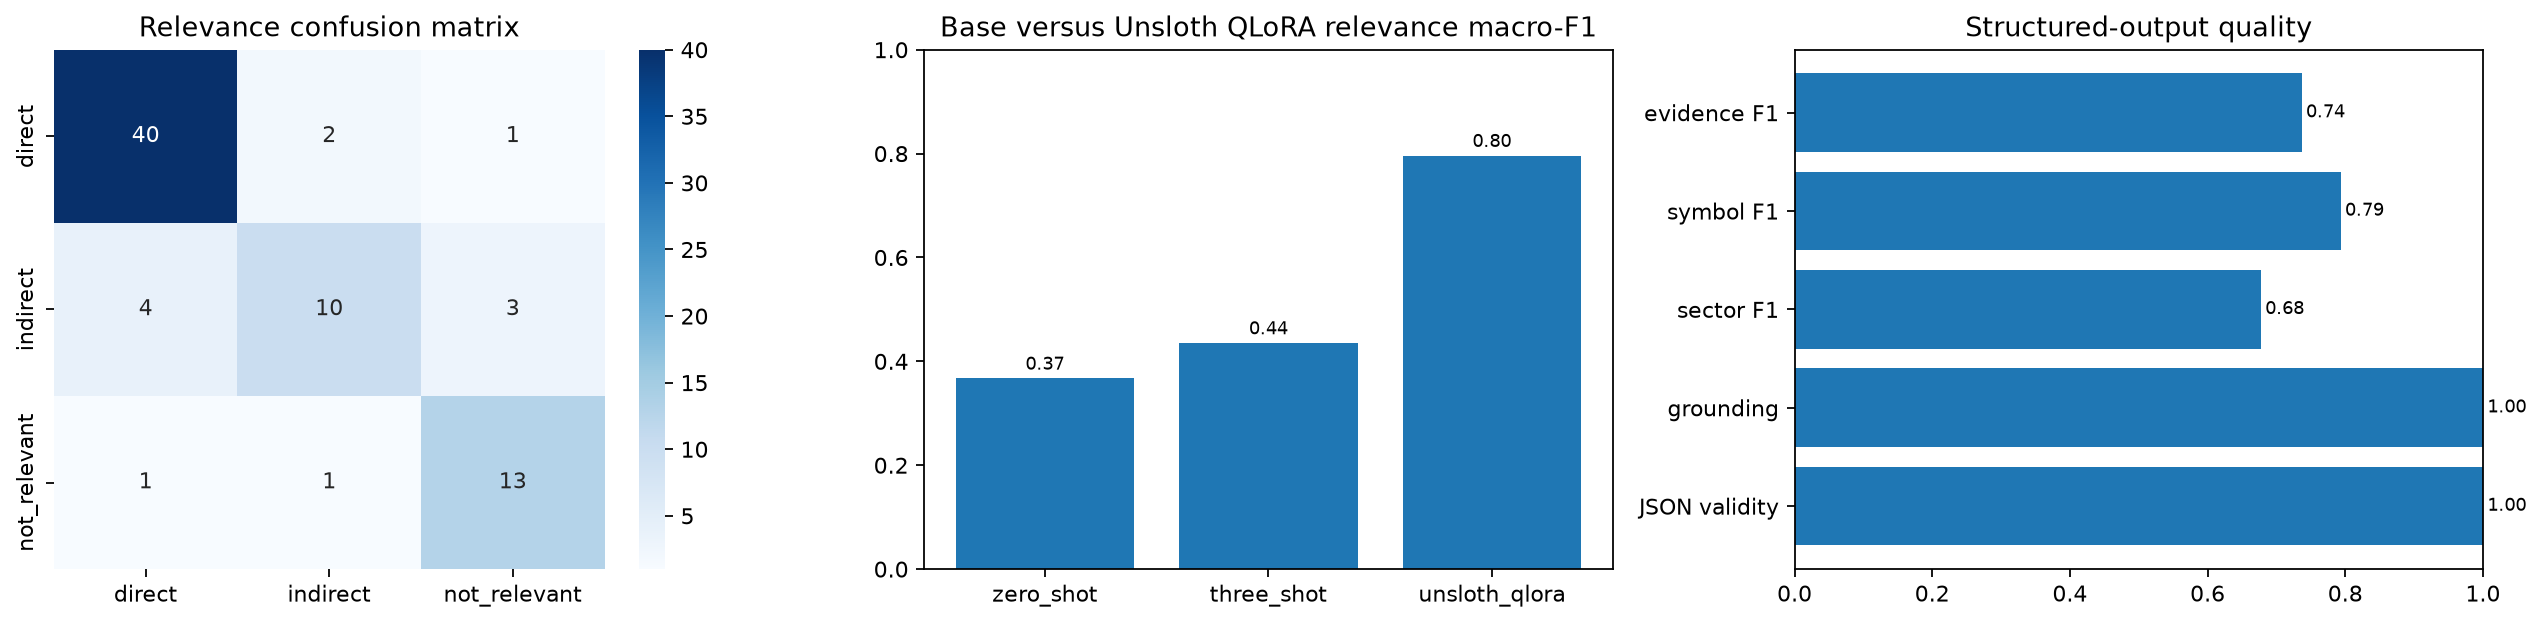
\includegraphics[width=0.96\textwidth]{assets/test_results.png}

  \vspace{0.12cm}
  \small Frozen-test diagnostic plot from the final Qwen3.5-9B targeted-v2 adapter artifact.
\end{frame}

\begin{frame}{Limitations and Future Work}
  \begin{columns}[T,onlytextwidth]
    \begin{column}{0.48\textwidth}
      \begin{alertblock}{Limitations}
        \begin{itemize}
          \item NEPSE-Impact-500 is small; rare events and neutral direction are under-covered, so standalone neutral cannot yet be learned.
          \item Historical market snapshots are partial.
          \item Set-valued sector, symbol, and evidence extraction show a recall gap.
          \item Lightning-hosted vLLM suits demos, not production deployment.
        \end{itemize}
      \end{alertblock}
    \end{column}
    \begin{column}{0.48\textwidth}
      \begin{block}{Future work}
        \begin{itemize}
          \item Expand and adjudicate neutral, sector-industry, regulation, and credit-financing hard cases to move beyond the merged target.
          \item Improve sector, symbol, and evidence recall via clearer selection rules and constrained post-processing.
          \item Complete independent second annotation and agreement metrics.
          \item Keep constrained inference and single-pass RAG while hardening deployment.
        \end{itemize}
      \end{block}
    \end{column}
  \end{columns}
\end{frame}

\begin{frame}{Conclusion}
  \begin{block}{Final contribution}
    MarketGyan delivers a Nepal-specific, evidence-grounded financial NLP research prototype with NEPSE-Impact-500, a Qwen3.5-9B targeted-v2 LoRA adapter, Qdrant evidence retrieval, and a live React/FastAPI/Node demonstration path.
  \end{block}

  \begin{itemize}
    \item The final model passes strict JSON validity and evidence grounding gates.
    \item Improved multilingual baselines: XLM-R relevance macro-F1 0.743 and merged-direction macro-F1 0.568 with no dead class.
    \item The frontend can demonstrate Ask MarketGyan, Evidence Search, and Reports.
    \item Deployment is not recommended until neutral direction and set-valued sector, symbol, and evidence recall improve.
  \end{itemize}

\end{frame}

\begin{frame}{References I}
  \tiny
  \begin{enumerate}
    \item D. Araci, ``FinBERT: Financial Sentiment Analysis with Pre-trained Language Models,'' arXiv:1908.10063, 2019.
    \item H. Yang et al., ``FinGPT: Open-Source Financial Large Language Models,'' arXiv:2306.06031, 2023.
    \item J. Lee, N. Stevens, S. C. Han, and M. Song, ``A Survey of Large Language Models in Finance,'' \emph{Neural Computing and Applications}, 2024.
    \item G. Bhatia et al., ``FinTral: A Family of GPT-4 Level Multimodal Financial Large Language Models,'' arXiv:2402.10986, 2024.
    \item S. Timilsina, M. Gautam, and B. Bhattarai, ``NepBERTa: Nepali Language Model Trained in a Large Corpus,'' AACL-IJCNLP, 2022.
    \item B. Subedi et al., ``Exploring the Potential of Large Language Models for Low-resource Languages: NER and POS Tagging for Nepali,'' LREC-COLING, 2024.
    \item P. Thapa et al., ``Development of Pre-Trained Transformer-based Models for the Nepali Language,'' CHiPSAL, 2025.
    \item E. J. Hu et al., ``LoRA: Low-Rank Adaptation of Large Language Models,'' ICLR, 2022.
    \item T. Dettmers et al., ``QLoRA: Efficient Finetuning of Quantized LLMs,'' NeurIPS, 2023.
  \end{enumerate}
\end{frame}

\begin{frame}{References II}
  \tiny
  \begin{enumerate}
    \setcounter{enumi}{9}
    \item P. Lewis et al., ``Retrieval-Augmented Generation for Knowledge-Intensive NLP Tasks,'' NeurIPS, 2020.
    \item T. Gao et al., ``Enabling Large Language Models to Generate Text with Citations,'' EMNLP, 2023.
    \item J. Zhang et al., ``LongCite: Enabling LLMs to Generate Fine-Grained Citations in Long-Context QA,'' arXiv:2409.02897, 2024.
    \item Qwen Team, ``Qwen3.5-9B Model Card,'' Hugging Face, 2026.
    \item vLLM Project, ``OpenAI-Compatible Server and Structured Outputs,'' 2026.
    \item Nepal Stock Exchange, ``NEPSE Market Data,'' 2026. \url{https://nepalstock.com/}
    \item ShareSansar, ``NEPSE Market and Index History Data,'' 2026. \url{https://www.sharesansar.com/}
    \item Nepal Rastra Bank, ``Notices, Publications, and Policy Documents,'' 2026. \url{https://www.nrb.org.np/}
    \item Securities Board of Nepal, ``Notices and Regulatory Publications,'' 2026. \url{https://www.sebon.gov.np/}
  \end{enumerate}
\end{frame}

\end{document}
